\chapter{色散}
\label{ch:Dispersion}

以下是上述内容的翻译:

在光学中,“色散”指的是光波在诸如玻璃等材料中的传播速度取决于这些波的时间频率。如果包含多种不同时间频率的光束以一定角度进入一块玻璃,则根据斯涅尔定律,这些组成频率将会在空间上分散开来~\cite{Snell}。如果一个具有一定持续时间、包含一系列时间频率的激光脉冲垂直进入同一块玻璃,则由于不同频率的光在传播过程中花费的时间不同,脉冲在另一端出来时可能会变长。本章将从基本原理出发,解释色散对激光脉冲的影响。

\section{脉冲和空间频率}

考虑公式 ~\ref{eq:pulse},假设脉冲在空间均匀介质中传播,因此 $\betag(z,\omega)=\betag(\omega)$,

\begin{align}
\label{eq:spatially_uniform}
    \E(z,t) &= \frac{1}{2\pi}\int_{-\infty}^{\infty} \Tilde{\E}(z,\omega) e^{i\betag(\omega)z-i\omega t} d\omega.
\end{align}

在介质中,$\betag(\omega)=n(\omega)\omega/c$,其中$n(\omega)$是材料的折射率,$c$是光速。对于光纤等波导来说,$\betag(\omega)$ 必须通过求解麦克斯韦方程来确定,如本 \href{https://youtu.be/z7fyT3etgis}{视频教程}中所述。此外,如图~\ref{fig:bandwidth} a)所示,本入门指南中考虑的脉冲包络的持续时间假定远远长于其载波频率下单次振荡的持续时间,即 $\omega_0/2\pi\approx 200$~THz。

\begin{figure}
    \centering
    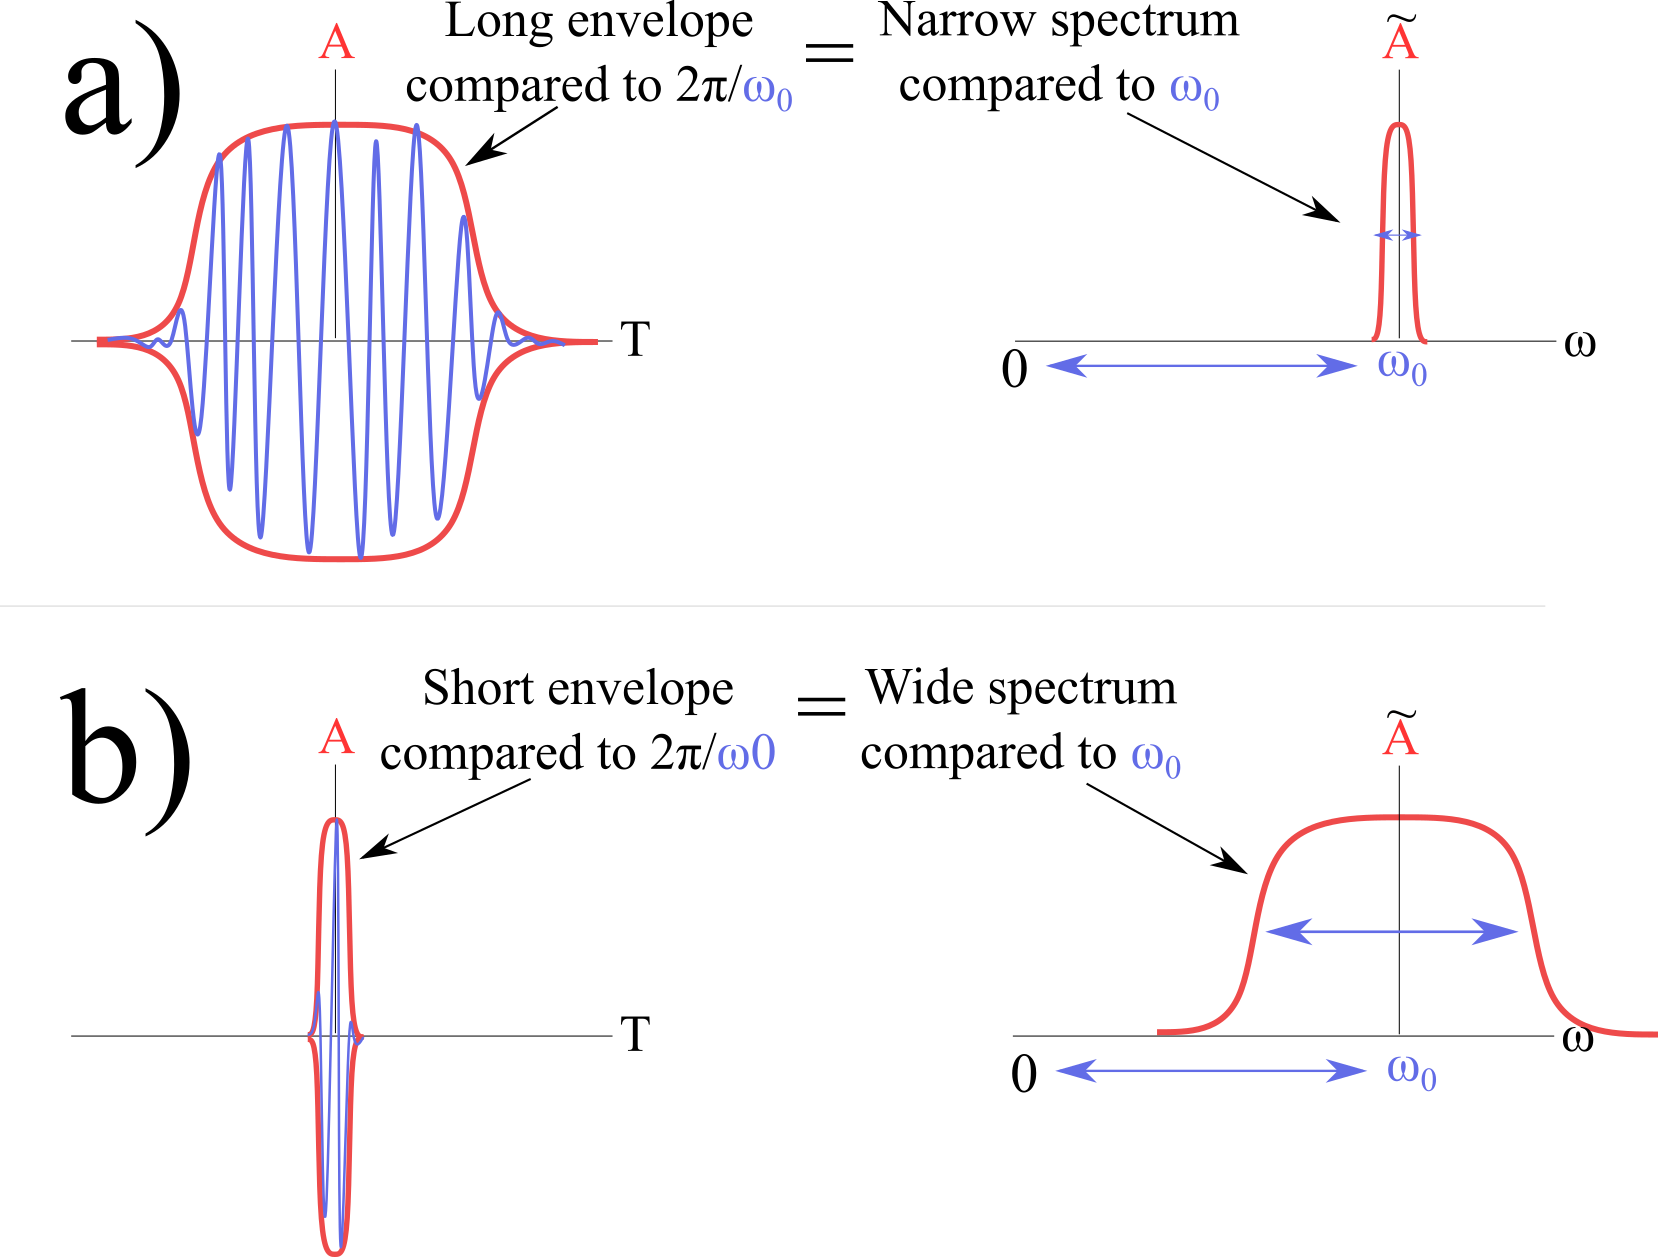
\includegraphics[width=1\linewidth]{figures/bandwidth.png}
    \caption{a) 与载波频率下单次电场振荡的持续时间相比,持续时间长的脉冲频谱较窄。 b)相反,短脉冲的频谱较宽。}
    \label{fig:bandwidth}
\end{figure}

根据这些假设,脉冲的频谱宽度非常窄,以至于 $\betag(\omega)$ 可以围绕载波频率泰勒展开为

\begin{align}
\label{eq:beta_approx}
    \betag(\omega)&\approx \betag(\omega_0)+\partial_\omega\betag|_{\omega_0}(\omega-\omega_0)+\frac{1}{2!}\partial^2_\omega\betag|_{\omega_0}(\omega-\omega_0)^2+
    \frac{1}{3!}\partial^3_\omega\betag|_{\omega_0}(\omega-\omega_0)^3+... \\ \nonumber
    &= \sum_{n=0}^{\infty} \frac{1}{n!}\partial^n_\omega\betag|_{\omega_0}(\omega-\omega_0)^n\\ \nonumber
    &=\sum_{n=0}^{\infty} \frac{1}{n!}\betag_n(\omega-\omega_0)^n.
\end{align}

考虑到这一简化,脉冲在介质中传播的表达式变为

\begin{align}
\label{eq:beta_approx_applied}
    \E(z,t) &= \frac{1}{2\pi}\int_{-\infty}^{\infty} \Tilde{\E}(z,\omega) e^{i(\betag_0+\betag_1(\omega-\omega_0)+\frac{1}{2}\betag_2(\omega-\omega_0)^2+...)z-i\omega t} d\omega.
\end{align}


\section{$\betag_0$ - 载波的延迟程度}

%Because the term containing $\betag_0$ does not depend on $\omega$, it can be moved outside the integral in Eq.~\ref{eq:beta_approx_applied}. Multiplying by $1=\exp(-i\omega_0t)\exp(i\omega_0t)$ yields
由于包含 $\betag_0$ 的项不依赖于 $\omega$,它可以移到公式 ~\ref{eq:beta_approx_applied} 的积分之外。乘以 $1=\exp(-i\omega_0t)\exp(i\omega_0t)$ 得到

\begin{align}
\label{eq:beta_approx_applied}
    \E(z,t) &= \frac{1}{2\pi} e^{i\betag_0z-i\omega_0t}  \int_{-\infty}^{\infty} \Tilde{\E}(z,\omega) e^{i(\betag_1(\omega-\omega_0)+\frac{1}{2}\betag_2(\omega-\omega_0)^2+...)z-i(\omega-\omega_0) t} d\omega.
\end{align}

积分外的指数意味着,如果观察介质中的复数电场,其持续时间为载波的几个周期,那么它看起来就像一个复数平面波,其时间频率为 $\omega_0$,空间频率为 $\betag_0$。关于 $\betag_0$ 对真实平面波在介质中传播的影响,请参见 \href{https://www.desmos.com/calculator/ausd1wnl2j}{此交互式图表}。

\subsection{相速度}
\label{sec:Phase_velocity}

当 $\betag_0z-\omega_0t$ 是 $2\pi$ 的整数倍时,载波将达到峰值。为简单起见,考虑与 $\betag_0z-\omega_0t=0$ 相对应的峰值。如果时间前进了 $0<Delta t$,$z$ 的原始值就不满足 $\betag_0z-\omega_0(t+\Delta t)=0$ 。相反,峰值会出现在某个新的位置 $z+\Delta z$,其中

\begin{align}
    \betag_0(z+\Delta z)-\omega_0(t+\Delta t)=0\\ \nonumber
    \betag_0\Delta z-\omega_0\Delta t=0.
\end{align}

由于峰值在 $\Delta t$ 时间内移动了 $\Delta z$,我们可以将 “相位速度”(或 “载波速度”)定义为

\begin{align}
\label{eq:Phase_velocity}
    v_p &= \frac{\Delta z}{\Delta t} = \frac{\omega_0}{\betag_0}.
\end{align}


\section{$\betag_1$ - 以载波为中心的脉冲包络延迟的程度}

式 ~\ref{eq:beta_approx_applied} 中的积分表示通过介质传播的复电场的包络。对指数项进行重排,可以得到

\begin{align}
\label{eq:envelope_beta1}
    \E(z,t) &= \frac{1}{2\pi} e^{i\betag_0z-i\omega_0t}  \int_{-\infty}^{\infty} \Tilde{\E}(z,\omega) e^{i\betag_1(\omega-\omega_0)z-i(\omega-\omega_0) t} e^{i(\frac{1}{2}\betag_2(\omega-\omega_0)^2+...)z} d\omega.
\end{align}

应用公式 ~\ref{eq:Phase_velocity} 后面的相同分析,我们会发现复电场包络的峰值以所谓的 “群速度”(或 “包络速度”)传播,其值为

\begin{align}
\label{eq:group_velocity}
    v_g &= \frac{(\omega-\omega_0)}{\betag_1\cdot(\omega-\omega_0)} = \frac{1}{\betag_1} = \frac{1}{\partial_\omega\betag}.
\end{align}

关于相位速度和群速度之间的区别,请参见 \href{https://www.desmos.com/calculator/rq2physwac}{此交互式图表}。请注意,公式~\ref{eq:group_velocity}与公式~\ref{eq:delay_definition}的预测一致,即相位相对于 $\omega$ 发生较大的正向变化应导致较大的延迟。




\section{$\betag_2$ - 构成以载波为中心的脉冲包络的频率相对延迟的程度}

\label{sec:GVD}

将公式 ~\ref{eq:envelope}应用于公式 ~\ref{eq:envelope_beta1},可以 “剔除 ”载波快速但可预测的空间和时间振荡,将注意力集中在包络上:

\begin{align}
    \A(z,t)  &= \frac{1}{2\pi}  \int_{-\infty}^{\infty} \Tilde{\A}(z,\omega) e^{i\betag_1(\omega-\omega_0)z-i(\omega-\omega_0) t} e^{i(\frac{1}{2}\betag_2(\omega-\omega_0)^2+...)z} d\omega.
\end{align}

为了进一步简化,我们可以定义 $T=t-\betag_1z$,即 “脉冲包络到达距离 $z$ 时的相对时间”。使用 $T$ 代替 $t$ 是很方便的,因为许多光学实验都需要发送脉冲光穿过固定长度的介质,并跟踪光离开介质后一段时间内测量到的功率:   

\begin{align}
    \A(z,T)  &= \frac{1}{2\pi}  \int_{-\infty}^{\infty} \Tilde{\A}(z,\omega) e^{i\betag_1(\omega-\omega_0)z-i(\omega-\omega_0) (T+\betag_1z)} e^{i(\frac{1}{2}\betag_2(\omega-\omega_0)^2+...)z} d\omega \\ \nonumber
    &= \frac{1}{2\pi}  \int_{-\infty}^{\infty} \Tilde{\A}(z,\omega) e^{i(\frac{1}{2}\betag_2(\omega-\omega_0)^2+...)z-i(\omega-\omega_0)T} d\omega.
\end{align} 

正如公式 ~\ref{eq:spectrum_time_example}所解释的那样,$\betag_2$ 的正值(负值)意味着较低的(较高的)时间频率比较高的(较低的)时间频率传播得更快,从而导致脉冲包络在时域中变宽。或者,我们也可以考虑只包含 $\betag_2$ 项的公式 ~\ref{eq:GNLSE}、

\begin{align}
    \label{eq:heat_equation}
    \partial_z \A = -i  \frac{\betag_2}{2}\partial_T^2\A,
\end{align}

这与所谓的 “热方程 ”相同 ~\cite{Fourier_heat_original,Fourier_heat_english}. 参见 
\href{https://digitalcommons.ursinus.edu/cgi/viewcontent.cgi?article=1008&context=triumphs_differ}{本教程}。为了得到 $\A(z,T)$ 给定的 $\A(z=0,T)$ 以及 $\tilde{A}(z=0,\omega)$ ,首先计算公式的傅立叶变换 ~\ref{eq:heat_equation} 以得到

\begin{align}
    \label{eq:beta2_broadening}
    \partial_z \Tilde{\A} &= -i  \frac{\betag_2}{2} (i(\omega-\omega_0))^2 \Tilde{\A} \\ \nonumber
    &= i  \frac{\betag_2}{2}(\omega-\omega_0)^2\Tilde{\A} \\ \nonumber
    \Tilde{\A}(z,\omega)&=\Tilde{\A}(0,\omega)e^{i\frac{\betag_2}{2}(\omega-\omega_0)^2z} \\ \nonumber
    \A(z,T) &= \IFT\left\{  \Tilde{\A}(z,\omega)   \right\}.
\end{align}

对于高斯脉冲,公式(~\ref{eq:beta2_broadening})可以通过(\href{https://drive.google.com/file/d/17Ab3bg0Hx0x8J-5lR29ejFg0eOlv6Psh/view?usp=sharing}{分析})求解。结果确实意味着脉冲会在时间上变宽,而将公式\ref{eq:chirp_definition}应用于结果则证实,$\betag_2>0$ 意味着低频将比高频更早到达。由于$\betag_2$引起的相位偏移的大小随着给定频率分量与载波之间距离的增加而呈二次增长,因此在相同距离内,频谱宽度较大的短脉冲将比带宽较小的短脉冲在时间上更宽。由 $\betag_2$ 导致的增宽变得显著的特征长度可定义为

\begin{align}
    \label{eq:Dispersion_length}
    L_{2} &= \frac{T_0^2}{|\betag_2|}.
\end{align}

有关色散对高斯脉冲的影响,请参阅 \href{https://www.youtube.com/watch?v=BP6Ra98AEuU}{本视频}。

\subsection{零色散频率}
\label{subsec:ZDF}

对于已知 $\betag(\omega)$ 的给定介质,可以计算出给定载波频率 $\omega_0$ 附近的 $\betag_2$ 值为

\begin{align}
\label{eq:ZDF}
    \betag_2(\omega) &= \betag_2|_{\omega=\omega_0} + \betag_3|_{\omega=\omega_0}\cdot(\omega-\omega_0)+\frac{1}{2}\betag_4|_{\omega=\omega_0}\cdot(\omega-\omega_0)^2 +...,
\end{align}

这样就可以求解特定频率(或者说复数频率!),$\omega_{ZD}$,其中$\betag_2(\omega_{ZD})=0$。这个 “零色散频率 ”非常重要,因为很多非线性机制在 $\omega_{ZD}$ 或接近 $\omega_{ZD}$ 的频率下会更有效,其中 $\betag_2<0$。因此,在进行非线性光学实验时,确定特定介质的 $\omega_{ZD}$ 值至关重要。特定光纤的零色散频率可以使用常见的光学实验室设备进行实验测量~\cite{zero_disp_measurement}。
从历史上看,用于电信的光纤被设计成接近激光的近红外频率($\approx$190-230~THz $\approx$1310-1550~nm),易于产生、调制和检测。这样做的目的是为了防止携带数字信息的脉冲出现时间展宽、重叠和干扰。自 2000 年代中期以来,电子色散补偿技术的进步使这种光纤设计变得过时甚至有害,因为非线性效应会通过改变信号的相位和振幅来扭曲信号,在接近 $\omega_{ZD}$ 时这种效应更为显著。

\section{$\betag_n$ - 高阶延迟}

在理解了$\betag(\omega)$(即$\betag_1$)的斜率决定脉冲包络的传播速度,而$\betag(\omega)$(即$\betag_2$)的曲率决定脉冲的时间展宽之后,这些见解可以得到推广。例如,$\betag_3>0$ 意味着$i\betag_3/6(\omega-\omega_0)^3z$ 项会导致除载波外所有频率的正$\partial_\omega\phi$。因此,对脉冲有贡献的高频和低频都会开始落后于主脉冲,从而导致不对称的时间展宽。此外,$\betag_4>0$意味着$i\betag_4/24(\omega-\omega_0)^4z$会在$\betag_2$引起的时间展宽之外引起额外的对称时间展宽。请参见图 ~\ref{fig:dispersion_combined},了解不同的 $\betag_n$ 项对高斯脉冲时间轮廓的影响。在分析脉冲在介质中传播的演化时,$\betag(\omega)$ 的扩展中包含多少项取决于脉冲的频谱宽度,而频谱宽度与其持续时间成反比。对于 1~ps 以上的脉冲,高于 $\betag_3$ 的阶数很少有贡献。在用持续时间为 10~fs 的脉冲对超连续产生进行数值模拟时,为了稳妥起见,通常会包含高达 $\betag_8$ 的阶次。与公式~\ref{eq:Dispersion_length}类似,高阶色散效应变得显著的特征长度定义为

\begin{align}
\label{eq:dispersion_length_general}
    L_{n} &= \frac{T_0^n}{|\betag_n|}.
\end{align}

有关色散的更多详情,请参阅 \href{https://www.youtube.com/watch?v=E3S0BQiy3p8&ab_channel=YourFavouriteTA}{本视频教程}。


\section{$\alpha(\omega)$ 和 $\betag(\omega)$ 是独立的吗?}
\label{sec:KK_relations}

在公式~\ref{eq:GNLSE}中,$\alpha$被视为常数,因为在典型脉冲的带宽范围内,其频率依赖性通常很弱。然而,原则上我们可以像对待 $\betag(\omega)$ 一样,对 $\alpha(\omega)$ 进行泰勒展开。有趣的是,我们发现对于给定介质来说,函数 $\alpha(\omega)$ 和 $\betag(\omega)$ 是通过所谓的 \href{https://en.wikipedia.org/wiki/Kramers%E2%80%93Kronig_relations#Related_proof_from_the_time_domain}{克莱默斯-克罗尼格关系(Kramers-Kronig Relations)} 相互关联的,知道其中一个就可以计算另一个。因此,$\alpha(\omega)$ 和 $\betag(\omega)$ 不能独立选择。从数学上证明这种联系很困难,但从物理上来说,直觉告诉我们,与频率相关的$\alpha(\omega)$吸收从根本上说正是产生与频率相关的相位延迟$\betag(\omega)$的原因。此外,介质在给定位置对外加电场的响应只能取决于该位置电场的当前和过去的值,这进一步限制了衰减和相位延迟的组合。方便的是,如果将 $\alpha(\omega)=\alpha$ 视为频率常数,那么它的值可以自由改变,而不会影响 $\betag_n$ 的任何值。 

有关克拉默-克罗尼格关系的更多详情,请参见 \href{https://www.youtube.com/watch?v=vzBnsG2rKWs}{视频一 } 和 \href{https://www.youtube.com/watch?v=rFTUTxPHYYw}{视频二}。请参阅 \href{https://www.desmos.com/calculator/1zymtgbbrv}{这个交互图},了解在时域中使用因果关系和克拉默-克罗尼格关系将 $\alpha(\omega)$ 与 $\betag(\omega)$ 联系起来的教程。


\begin{figure}
    \centering
    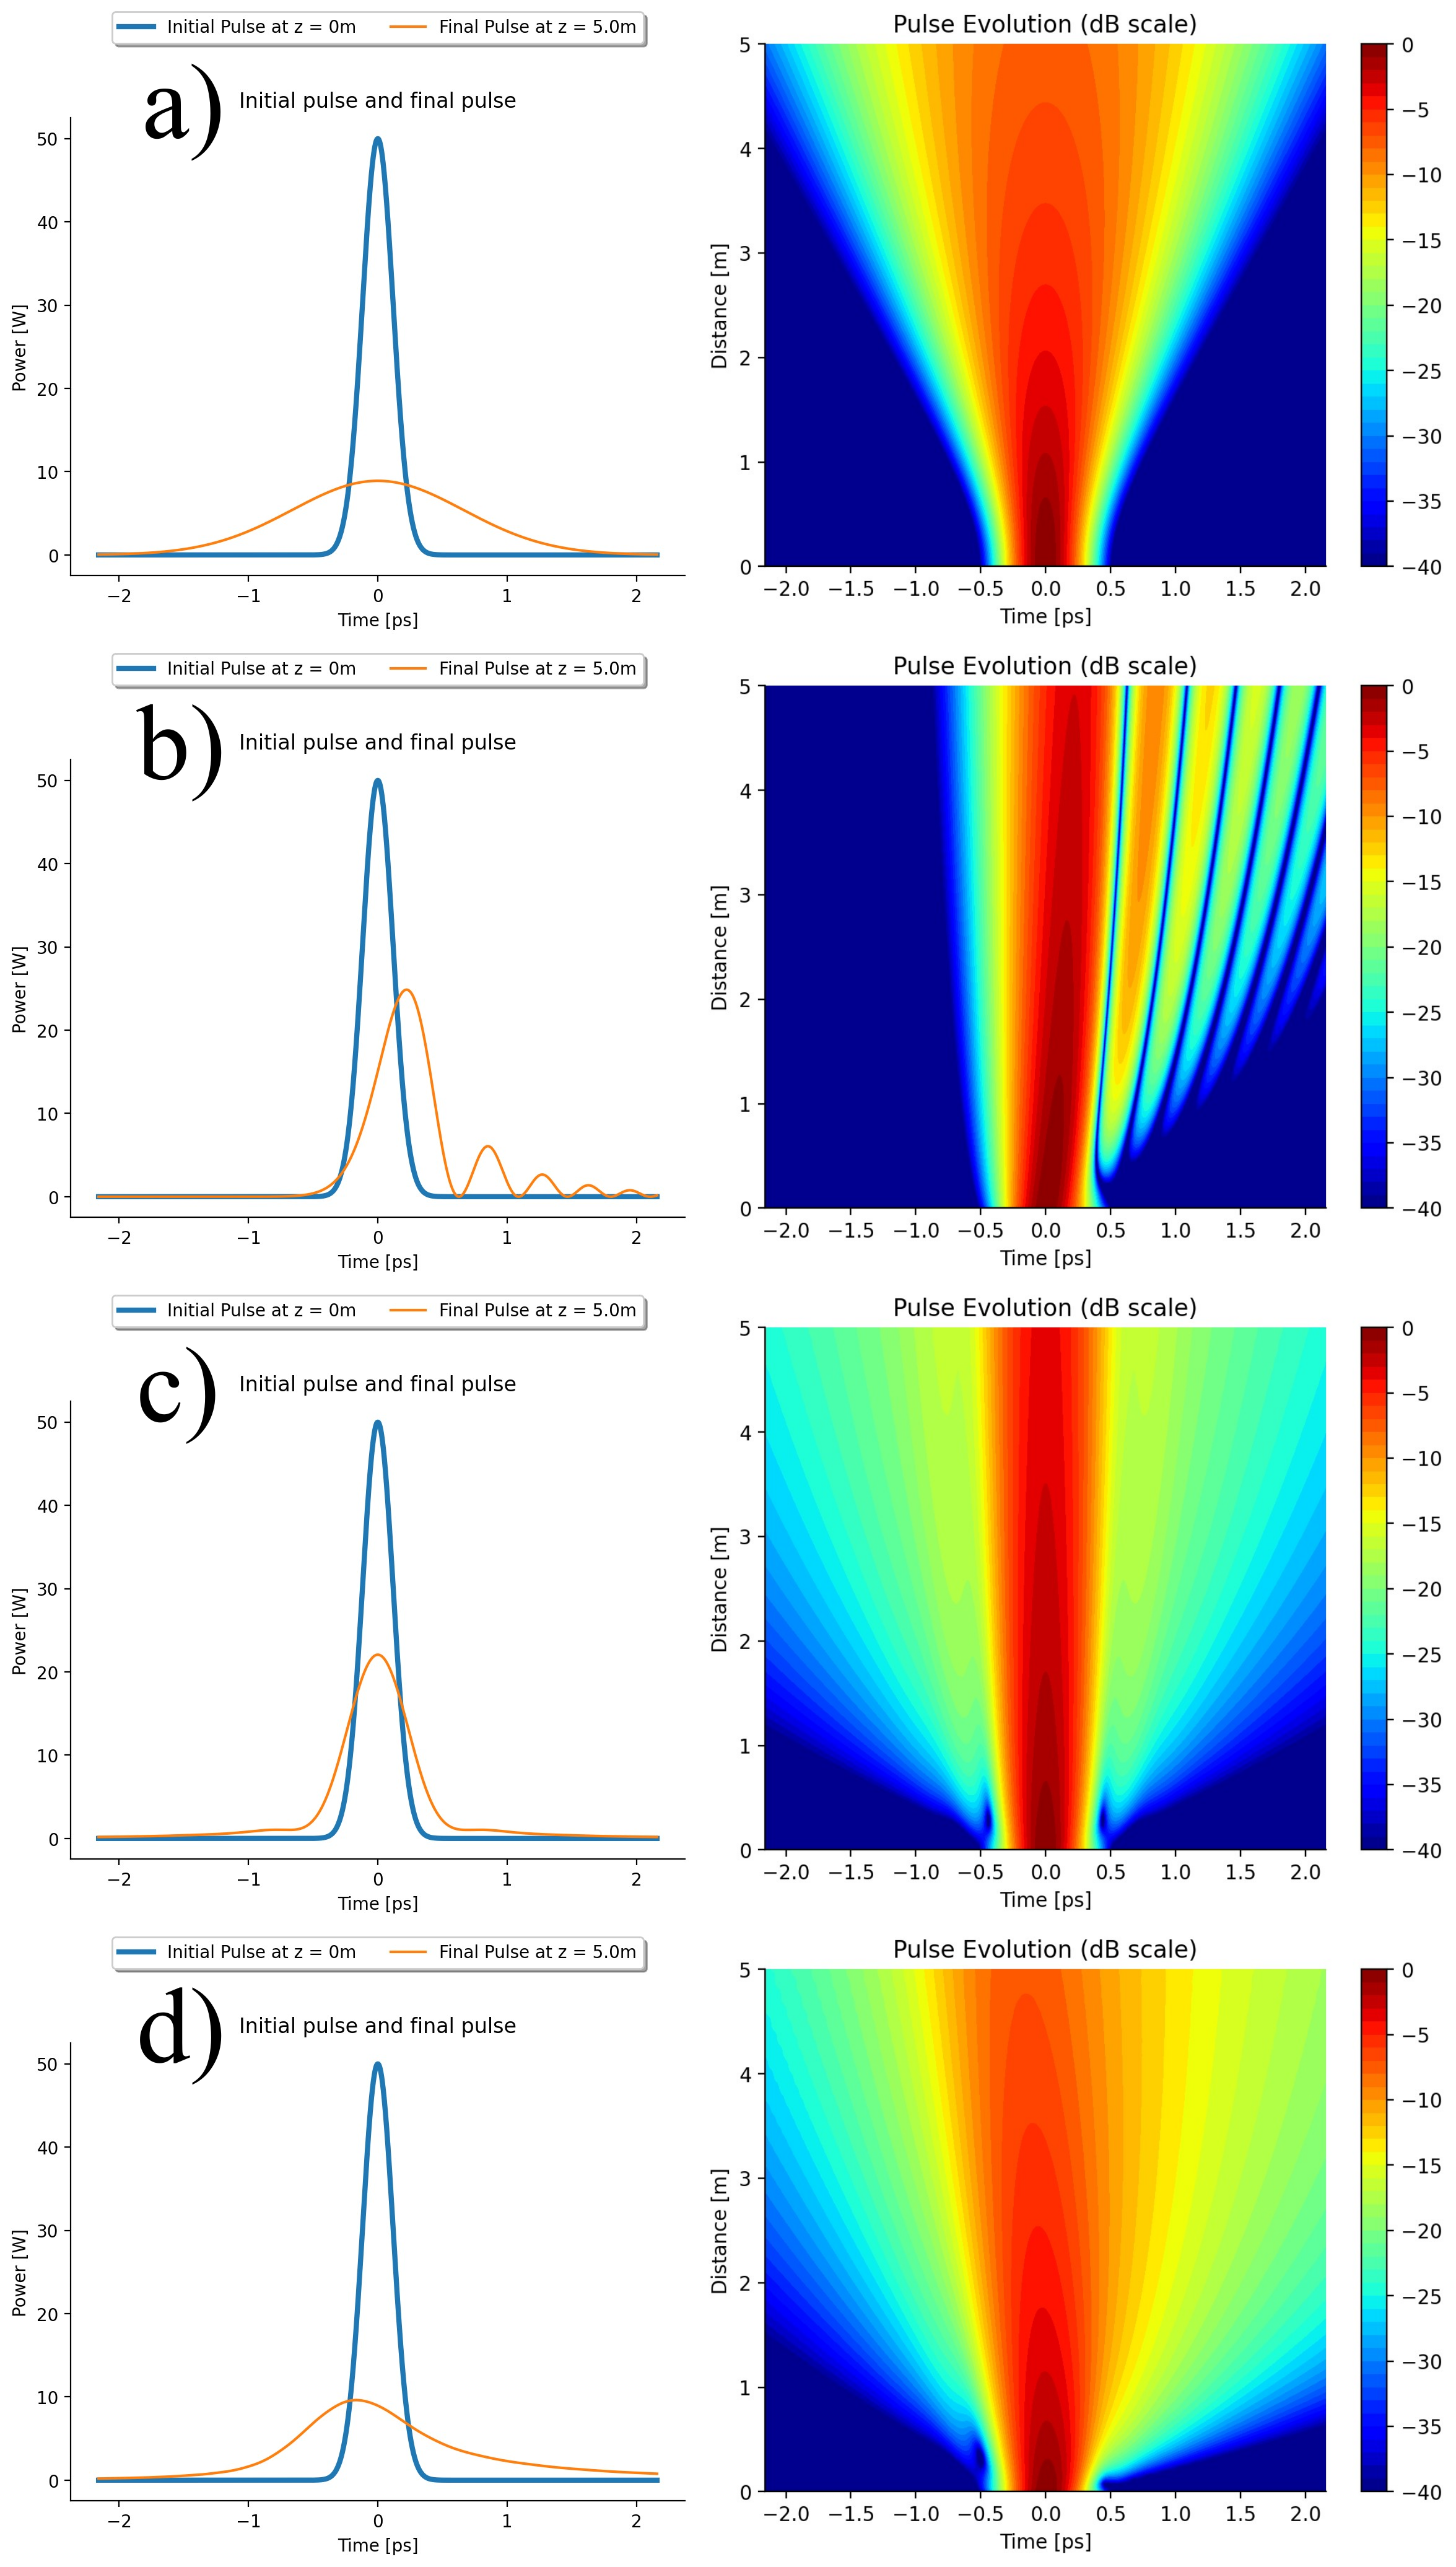
\includegraphics[width=0.75\linewidth]{figures/dispersion_combined.png}
    \caption{时域中不同 $\betag_n$ 项对高斯脉冲的影响说明。左栏显示了脉冲在不同$\betag_n$项介质中传播前后的功率包络对比。右栏显示的是功率包络随距离的变化。  a) $\betag_2<0$ 的介质; b) $\betag_3>0$ 的介质; c) $\betag_4<0$ 的介质; d) 同时存在 $\betag_2<0$ 、 $\betag_3>0$ 和 $\betag_4<0$ 的介质。
    使用 \href{https://colab.research.google.com/drive/1PW9smFA3PECvcXyWpZcW1ogY4W3hEYFt?usp=sharing}{这个可交互notebook} 中的数值模拟生成。我们鼓励读者尝试使用。}
    \label{fig:dispersion_combined}
\end{figure}